\documentclass[11pt,a4paper]{article}
\usepackage[utf8]{inputenc}
\usepackage{amsmath,amssymb,amsfonts}
\usepackage{booktabs}
\usepackage{graphicx}
\usepackage{float}
\usepackage{caption}
\usepackage{xcolor}
\usepackage{tikz}
\usetikzlibrary{positioning,arrows.meta,fit,backgrounds}
\usepackage{microtype}
\usepackage[bookmarks=true,pdfencoding=auto]{hyperref}

\hypersetup{
    colorlinks=true,
    linkcolor=blue!75!black,
    urlcolor=blue!75!black,
    citecolor=blue!75!black,
    pdftitle={From Hard Thresholds to Differentiable Binarization: The Mathematics of DBNet},
    pdfauthor={Nguyen Dang Long},
    pdfsubject={Mathematical derivation of the DBNet scene-text detection algorithm},
    pdfkeywords={scene text detection, differentiable binarization, DBNet, affinity map, semantic segmentation}
}

% ------------------------------------------------------------------------------
% Page geometry and compact typography
% ------------------------------------------------------------------------------
\setlength{\textwidth}{6.75in}
\setlength{\textheight}{9.5in}
\setlength{\oddsidemargin}{-0.125in}
\setlength{\evensidemargin}{-0.125in}
\setlength{\topmargin}{-0.65in}
\setlength{\headheight}{12pt}
\setlength{\headsep}{12pt}
\setlength{\footskip}{22pt}

\setlength{\parindent}{0pt}
\setlength{\parskip}{3pt plus 1pt minus 0.5pt}

\setlength{\abovedisplayskip}{4.5pt plus 2pt minus 1.5pt}
\setlength{\belowdisplayskip}{4.5pt plus 2pt minus 1.5pt}
\setlength{\abovedisplayshortskip}{2.5pt plus 1pt minus 1pt}
\setlength{\belowdisplayshortskip}{2.5pt plus 1pt minus 1pt}

\makeatletter
\def\tightlist{%
  \setlength{\itemsep}{1.5pt}%
  \setlength{\parsep}{0pt}%
  \setlength{\topsep}{2pt}%
  \setlength{\partopsep}{0pt}%
}
\let\olditemize\itemize
\def\itemize{\olditemize\tightlist}
\let\oldenumerate\enumerate
\def\enumerate{\oldenumerate\tightlist}

\renewcommand\section{\@startsection {section}{1}{\z@}%
                                   {-2.0ex \@plus -0.5ex \@minus -.2ex}%
                                   {0.8ex \@plus.2ex}%
                                   {\normalfont\large\bfseries}}
\renewcommand\subsection{\@startsection{subsection}{2}{\z@}%
                                     {-1.4ex\@plus -0.4ex \@minus -.2ex}%
                                     {0.5ex \@plus .2ex}%
                                     {\normalfont\normalsize\bfseries}}
\makeatother

\definecolor{boxbg}{HTML}{F8FAFC}
\definecolor{boxborder}{HTML}{2B6CB0}
\newcommand{\keybox}[1]{%
    \par\vspace{2pt}%
    \noindent\fcolorbox{boxborder}{boxbg}{%
        \begin{minipage}{\dimexpr\textwidth-2\fboxsep-2\fboxrule\relax}
            \vspace{1.5pt}#1\vspace{1.5pt}
        \end{minipage}%
    }%
    \par\vspace{2pt}%
}

\renewcommand{\labelitemi}{$\bullet$}
\renewcommand{\labelitemii}{--}
\newcommand{\code}[1]{\texttt{\detokenize{#1}}}
\newcommand{\rc}[1]{{\raggedright #1\par}}

\newcommand{\1}{\mathbf{1}}

\title{\textbf{From Hard Thresholds to Differentiable Binarization} \\
\large The Mathematics of Real-Time Scene Text Detection (DBNet)}
\author{\textbf{Nguyen Dang Long} \\ \texttt{vincentlalo-long}}
\date{November 2026}

\begin{document}
\maketitle

\begin{abstract}
Real-time scene text detection requires converting continuous probability predictions into discrete bounding polygons. Conventional segmentation pipelines apply heuristic, hard thresholding during post-processing, severing gradient propagation and creating an uncalibrated train-test mismatch under visual distribution shifts. This paper provides a first-principles mathematical analysis of Differentiable Binarization (DBNet). We formalize text detection as dense binary prediction, examine why standard scalar thresholding and Straight-Through Estimators (STE) fail, and derive the exact forward and backward dynamics of the Differentiable Binarization operator. Furthermore, we analyze adaptive threshold map generation, distance-transform-based affinity map supervision, and polygon decoding geometry. Finally, we evaluate the theoretical failure modes, instance-level confidence calibration, and geometric trade-offs governing real-time scene text extraction.
\end{abstract}

% ==============================================================================
\section{Classical Semantic Segmentation: Principles and the Post-Processing Pipeline}
% ==============================================================================

\subsection{Dense Pixel-Level Classification Formulation}
In classical computer vision, dense segmentation frameworks (such as FCN~\cite{fcn}, U-Net~\cite{unet}, and Mask R-CNN~\cite{maskrcnn}) formulate object localization as a dense pixel-level classification task. Rather than directly predicting parametric bounding geometries $(x, y, w, h, \theta)$, the model is tasked with answering a localized hypothesis at every spatial coordinate $(x,y)$: \emph{``Does pixel $(x,y)$ belong to an object instance or background scenery?''}

For scene text detection, the objective simplifies to dense binary segmentation over the spatial image lattice $\Omega = \{1,\dots,H\} \times \{1,\dots,W\}$:
\keybox{\textbf{Notation.} Let $I \in \mathbb{R}^{H \times W \times 3}$ denote the input image; $p(x,y) \in [0,1]$ is the model's predicted foreground probability at pixel $(x,y)$; $y(x,y) \in \{0,1\}$ is the ground-truth binary label; $P, Y \in [0,1]^{H' \times W'}$ denote the corresponding full-lattice probability and label maps; $d((x,y), C)$ represents the Euclidean distance from $(x,y)$ to a contour $C$; $\sigma(t) = 1/(1+e^{-t})$ is the standard logistic sigmoid function; and $\1[\cdot]$ denotes the indicator function.}

\subsection{The Encoder--Decoder Paradigm: Receptive Field vs.\ Boundary Precision}
To classify dense pixels without suffering prohibitive computational complexity $\mathcal{O}(H \times W)$ across deep feature spaces, architectures employ an asymmetric funnel topology:
\begin{enumerate}
    \item \textbf{Encoder (Hierarchical Abstraction and Downsampling):} A convolutional backbone $E_\phi$ systematically reduces spatial dimensions through strided convolutions or max-pooling layers:
    \[
    \mathbf{X}_0 = I \in \mathbb{R}^{H \times W \times 3} \;\xrightarrow{E_\phi}\; \mathbf{X}_l \in \mathbb{R}^{\frac{H}{2^l} \times \frac{W}{2^l} \times C_l}, \quad l \in \{1, \dots, L\}.
    \]
    Each downsampling step expands the effective receptive field (ERF) at layer $l$:
    \begin{equation}
    R_l = R_{l-1} + (k_l - 1) \prod_{i=1}^{l-1} s_i,
    \label{eq:erf}
    \end{equation}
    where $k_l$ and $s_i$ denote kernel sizes and operational strides. While a large receptive field is essential for contextual semantic disambiguation (e.g., distinguishing text glyphs from complex background clutter), it incurs a severe loss of high-frequency spatial detail, blurring boundary edges and stroke corners.
    \item \textbf{Skip Connections and Lateral Feature Fusion:} To recover lost spatial fidelity, architectures employ lateral skip pathways (e.g., channel concatenation in U-Net~\cite{unet}, or $1{\times}1$ projection combined with elementwise addition in Feature Pyramid Networks (FPN)~\cite{fpn}):
    \begin{equation}
    \mathbf{F}_l = \operatorname{Conv}_{3\times 3}\!\Big( \operatorname{Proj}_{1\times 1}(\mathbf{X}_l) + \operatorname{Upsample}_{2\times}(\mathbf{F}_{l+1}) \Big),
    \label{eq:fpn-fusion}
    \end{equation}
    fusing high-level semantic abstractions with low-level, high-resolution edge features.
    \item \textbf{Decoder (Spatial Resolution Recovery):} The decoder progressively reconstructs spatial dimensions via bilinear interpolation or transposed convolutions ($\mathcal{W}^\top * \mathbf{X}$), projecting the fused representation to an operating resolution $H' \times W'$ (typically $H/4 \times W/4$ for real-time throughput).
\end{enumerate}

\subsection{Dense Probability Modeling and Objective Formulations}
At the terminal decoder layer, a $1{\times}1$ convolution coupled with a sigmoid activation emits a continuous probability map:
\begin{equation}
P = \sigma\!\left(f_\theta(I)\right) \in [0,1]^{H' \times W'}, \qquad p(x,y) = \frac{1}{1 + \exp\left(-f_\theta(I)(x,y)\right)}.
\label{eq:prob-map}
\end{equation}
Supervision compares the continuous prediction $P$ against ground-truth raster masks $Y \in \{0, 1\}^{H' \times W'}$. Because text strokes typically occupy a negligible fraction of the image canvas ($\sum Y \ll H'W'$), standard cross-entropy suffers catastrophic class-imbalance collapse. Training therefore relies on composite loss objectives:
\begin{enumerate}
    \item \textbf{Weighted / $\alpha$-Balanced Cross-Entropy (BCE):}
    \begin{equation}
    \mathcal{L}_{\mathrm{BCE}}(P, Y)
      = -\frac{1}{N} \sum_{(x,y)} w(x,y)
        \Big[ \alpha\, y \log p + (1-\alpha)(1-y)\log(1-p) \Big],
    \label{eq:bce}
    \end{equation}
    with $\alpha \in (0,1)$ (typically $\alpha = 0.7$, upweighting rare positive text pixels) and a spatial weight map $w(x,y) \ge 0$ designed to downweight ambiguous boundary bands.
    \item \textbf{Soft Dice Loss (Continuous Set Intersection):} While BCE evaluates pixels independently, region-level losses optimize geometric set agreement. The soft Dice loss treats $P$ and $Y$ as fuzzy continuous sets~\cite{dice}:
    \begin{equation}
    \mathcal{L}_{\mathrm{dice}}(P, Y)
      = 1 - \frac{2 \sum_{(x,y)} p(x,y)\, y(x,y) + \varepsilon}{\sum_{(x,y)} p(x,y) + \sum_{(x,y)} y(x,y) + \varepsilon},
    \label{eq:dice}
    \end{equation}
    where $\varepsilon > 0$ prevents division by zero in all-background scenes; DBNet adopts this linear form (with binary labels $\sum y^2 = \sum y$, the squared variant of generalized Dice differs only in the prediction term). Differentiating with respect to $p(x,y)$, with $N = 2\sum p\,y + \varepsilon$ and $D = \sum p + \sum y + \varepsilon$,
    \begin{equation}
    \frac{\partial \mathcal{L}_{\mathrm{dice}}}{\partial p(x,y)}
      = \frac{N - 2\, y(x,y)\, D}{D^{2}},
    \label{eq:dice-grad}
    \end{equation}
    which penalizes each pixel in proportion to its overlap contribution versus the global region masses.
\end{enumerate}
The segmentation objective combines both terms: $\mathcal{L}_{\mathrm{seg}} = \mathcal{L}_{\mathrm{dice}} + \mathcal{L}_{\mathrm{BCE}}$.

\subsection{The Classical Post-Processing Pipeline: From Rasters to Geometric Instances}
A fundamental limitation of traditional segmentation is that the neural network halts at the continuous raster map $P$. Extracting concrete instances (e.g., bounding boxes or bounding polygons) is offloaded entirely to a sequence of heuristic, external image-processing algorithms executed on the host CPU:

\begin{figure}[H]
\centering
\begin{tikzpicture}[
  >={Latex[length=2mm]},
  stepnode/.style={draw=blue!60!black, fill=blue!5, rounded corners=3pt, align=center, font=\small, minimum height=8mm, text width=6.5cm},
  resnode/.style={draw=orange!65!black, fill=orange!8, rounded corners=3pt, align=center, font=\small, minimum height=8mm, text width=6.5cm},
  arrlabel/.style={font=\scriptsize, text=black!75, align=left}
]
\node[stepnode] (prob) {\textbf{Probability Map} $P \in [0,1]^{H' \times W'}$};
\node[stepnode, below=0.6cm of prob] (bin) {\textbf{Static Binarization}\\$B(x,y) = \1\!\left[ p(x,y) \ge \tau_0 \right]$};
\node[stepnode, below=0.6cm of bin] (morph) {\textbf{Morphological Regularization}\\Opening ($B \circ K$) / Closing ($B \bullet K$)};
\node[stepnode, below=0.6cm of morph] (trace) {\textbf{Topological Border Following}\\Suzuki--Abe Algorithm (\code{cv2.findContours})};
\node[resnode, below=0.6cm of trace] (geom) {\textbf{Geometric Fitting}\\Minimum-Area Rectangles / Polygons $\{\mathcal{R}_k\}$};

\draw[->, thick] (prob) -- node[right=0.2cm, arrlabel] {Global scalar threshold ($\tau_0 = 0.5$)} (bin);
\draw[->, thick] (bin) -- node[right=0.2cm, arrlabel] {Structuring element $K$ (Dilation / Erosion)} (morph);
\draw[->, thick] (morph) -- node[right=0.2cm, arrlabel] {Connected components $\{\mathcal{C}_k\}$} (trace);
\draw[->, thick] (trace) -- node[right=0.2cm, arrlabel] {Rotating calipers ($\min \mathrm{Area}(\mathcal{R})$)} (geom);
\end{tikzpicture}
\caption{The classical multi-stage post-processing pipeline bridging continuous segmentation probabilities to discrete bounding instances.}
\label{fig:classical-pipeline}
\end{figure}

The traditional pipeline executes in four sequential stages:
\begin{enumerate}
    \item \textbf{Global Scalar Thresholding:} The continuous map $P$ is converted into a binary mask $B(x,y)$ by applying a static scalar cutoff $\tau_0 \in (0,1)$ (conventionally $\tau_0 = 0.5$):
    \begin{equation}
    B(x,y) = \1\!\left[ p(x,y) \ge \tau_0 \right] =
    \begin{cases}
    1, & p(x,y) \ge \tau_0, \\
    0, & p(x,y) < \tau_0.
    \end{cases}
    \label{eq:static-bin}
    \end{equation}
    \item \textbf{Morphological Regularization:} Binary masks are filtered using structuring elements $K \in \{0, 1\}^{m \times m}$ to eliminate isolated stroke artifacts via morphological opening $B \circ K = (B \ominus K) \oplus K$ and close internal stroke perforations via morphological closing $B \bullet K = (B \oplus K) \ominus K$.
    \item \textbf{Topological Border Following (Suzuki--Abe Algorithm):} Connected components of foreground pixels ($B=1$) are traced into vector boundary polygons using hierarchical border-following algorithms (Suzuki \& Abe, 1985~\cite{suzuki}; standard \code{cv2.findContours}). The algorithm scans raster rows, identifies 0-to-1 boundary transitions, and traces 8-connected borders to emit ordered coordinate loops $\mathcal{C}_k = \{(x_i, y_i)\}_{i=1}^{M_k}$.
    \item \textbf{Geometric Fitting:} For each traced contour $\mathcal{C}_k$, an enclosing geometric primitive is fitted:
    \[
    \mathcal{R}_k^* = \arg\min_{\mathcal{R}} \operatorname{Area}(\mathcal{R}) \quad \text{s.t.} \quad \mathcal{C}_k \subseteq \mathcal{R},
    \]
    typically solved via Freeman's rotating calipers algorithm to produce minimum-area bounding rectangles or oriented quadrilaterals.
\end{enumerate}

\subsection{The Scene Text Dilemma: Three Structural Breakdowns}
When applied to scene text detection in video frames or complex natural scenes, this classical paradigm breaks down due to three fundamental structural failures:
\begin{enumerate}
    \item \textbf{Text Clumping and Inter-Glyph Coalescence:} Typographic text features extremely dense character kerning, where the spatial spacing between consecutive glyphs $\Delta x$ is often on the order of 1--3 pixels. Strided downsampling in the encoder and convolutional spatial smoothing blur these delicate gaps. Consequently, the inter-character background pixels exhibit ambiguous probabilities hovering in the range $p(x,y) \in [0.4, 0.6]$. Under a global threshold $\tau_0 = 0.5$, the binarizer bridges the gap between adjacent letters and adjacent lines, fusing entire words, phrases, or paragraphs into an intractable, monolithic connected component. Once merged into a single topological contour, downstream geometric fitting is powerless to separate individual text instances.
    \item \textbf{Gradient Disconnection and Optimization Blindness:} The neural network is optimized purely for pixel-level likelihoods $P$, completely decoupled from the geometric quality of the resulting bounding boxes $\mathcal{R}_k$. The binarization step \eqref{eq:static-bin} and border-following operator are piecewise-constant step mappings whose classical derivatives with respect to $P$ vanish almost everywhere:
    \begin{equation}
    \frac{\partial B(x,y)}{\partial p(x,y)} = \delta\!\left(p(x,y) - \tau_0\right) = 0 \quad \text{almost everywhere}.
    \label{eq:vanished-grad}
    \end{equation}
    Because the gradient path is severed, errors committed during polygon fitting (e.g., loose boundaries, merged words, or truncated punctuation) cannot transmit supervisory gradient feedback to adjust the weights of the convolutional backbone. The network remains fundamentally blind to instance-level geometric errors.
    \item \textbf{Computational Latency and Real-Time Infeasibility:} Morphological operations require $\mathcal{O}(H \times W \times |K|)$ serial pixel passes, and topological contour tracing (Suzuki--Abe) relies on sequential raster scanning with pointer-chasing memory patterns that cannot be parallelized on GPU or SIMD vector hardware. On high-resolution video streams (e.g., 720p or 1080p), serial CPU-bound post-processing consumes 50--200\,ms per frame, single-handedly preventing the pipeline from achieving real-time throughput ($>30$\,FPS).
\end{enumerate}

% ==============================================================================
\section{The Binarization Dilemma: From Heuristic Cuts to Differentiable Surrogates}
% ==============================================================================

\subsection{Why Static Scalar Thresholding Fails Under Distribution Shift}
A continuous probability map is not a terminal detection output: contours, polygons, and text lines are computed from a \emph{binary} representation. The classical mapping operator is the Heaviside step function:
\begin{equation}
B(x,y) = \1\!\left[ p(x,y) > \tau \right],
\label{eq:heaviside}
\end{equation}
for some scalar threshold $\tau$. In classical edge detection, this formulation mirrors the Canny operator~\cite{canny}, which convolves with Gaussian derivatives $G_\sigma$, computes the gradient magnitude $g$, and thresholds $g$ via a hysteresis pair $(\tau_\ell, \tau_h)$. The threshold is an unlearned, hand-tuned scalar.

When applied to deep neural probability maps, static scalar thresholding causes two catastrophic failure modes:
\begin{enumerate}
    \item \textbf{Distribution shift under variable illumination and font geometry.} The empirical mean, dynamic range, and variance of $p(x,y)$ shift radically across distinct image samples due to variations in ambient lighting, motion blur, font weight, compression artifacts, and background contrast. A fixed scalar $\tau_0 = 0.5$ is fundamentally uncalibrated for any image whose posterior response does not align with the training distribution's empirical center. Conventional inference systems resort to ad-hoc, per-image or per-batch normalization ($p / \max(p)$)---an unlearned, fragile heuristic that fails under noisy outliers.
    \item \textbf{Vanished gradients and optimization blockage.} The classical derivative of the Heaviside step is zero everywhere except at the singular boundary $p = \tau$:
    \[
    \frac{\partial B}{\partial p} = \delta(p - \tau) = 0 \quad \text{for } p \ne \tau.
    \]
    The mapping \eqref{eq:heaviside} completely discards all first-order gradient information regarding \emph{how close} a borderline pixel lies to the decision boundary. While the neural network can be trained to minimize pixelwise loss on $p$, the downstream binarized output depends on a discontinuous function that backpropagation cannot penetrate.
\end{enumerate}

\keybox{\textbf{The binarization gap in one sentence.} Neural training optimizes a continuous probability field $P$; downstream geometry consumes a discrete binary lattice $B$; every bridge between the two that is omitted from the computational graph introduces an intractable train-test discrepancy.}

\subsection{Straight-Through Estimators: Bypassing, Not Solving}
A widespread workaround adapted from quantized neural networks is the Straight-Through Estimator (STE)~\cite{ste}. The STE executes the exact discontinuous step \eqref{eq:heaviside} during the forward pass, but substitutes an identity gradient operator during backpropagation:
\begin{equation}
\frac{\partial \mathcal{L}}{\partial p} \Big|_{\mathrm{STE}} \;:=\; \frac{\partial \mathcal{L}}{\partial B}.
\label{eq:ste}
\end{equation}
While the STE prevents gradient starvation, the resulting gradient signal is fundamentally unfaithful to the underlying geometry:
\begin{enumerate}
    \item It instructs every pixel to uniformly push $p$ upward or downward regardless of whether $p$ lies adjacent to the decision level set $p \approx \tau$ or deep within the interior of a background region.
    \item Because the scalar $\tau$ does not participate in any differentiable mathematical expression, the STE provides no analytical mechanism to learn or adjust the threshold $\tau$ itself.
\end{enumerate}

Differentiable Binarization (DBNet)~\cite{dbnet} addresses both dilemmas in a unified, mathematically rigorous formulation: rather than forcing the network to adapt to an external heuristic threshold, the binarization operator is lifted directly into the differentiable computational graph.

% ==============================================================================
\section{Differentiable binarization (DB)}
% ==============================================================================

\subsection{The DB layer}
DB keeps the shape of \eqref{eq:heaviside}---a comparison between the probability map and a threshold---but makes two changes simultaneously:
\begin{enumerate}
    \item the threshold $\tau$ becomes a \emph{predicted, per-pixel map} $\tau(x,y)$ produced by a second convolutional branch;
    \item the step function is replaced by a steep sigmoid, so the comparison is inside the computation graph.
\end{enumerate}
The binarized output is
\begin{equation}
P^{d} = \sigma\!\big( \gamma (P - \tau) \big), \qquad \gamma \gg 1,
\label{eq:db}
\end{equation}
with $\gamma$ a scale hyperparameter (order $10^3$). Equation~\eqref{eq:db} is the entire method; everything below is analysis of its consequences.

\subsection{It is still a binarizer}
For any pixel with $p \ne \tau$,
\[
\lim_{\gamma \to \infty} \sigma\!\big( \gamma (p - \tau) \big) = \1[p > \tau],
\]
so $\eqref{eq:db}$ is a smooth one-parameter family converging pointwise to the hard decision of \eqref{eq:heaviside}. At inference, implementations apply \eqref{eq:db} with large $\gamma$ and then threshold at $0.5$, which by $\sigma(t) > 0.5 \iff t > 0$ is \emph{exactly} the event $p > \tau(x,y)$. Train and inference compute the same decision; $\gamma$ controls only the sharpness of the surrogate used for gradients, in the same way temperature controls the sharpness of a softmax.

\subsection{Gradient analysis}
With $s := P^{d} = \sigma(\gamma(p - \tau))$,
\[
\frac{\partial s}{\partial t} = \gamma\, s (1-s) \quad \text{for } t = p \text{ or } t = \tau,
\]
hence by the chain rule
\begin{align}
\frac{\partial \mathcal{L}}{\partial p}
  &= \frac{\partial \mathcal{L}}{\partial s}\; \gamma\, s (1-s),
   \label{eq:grad-p}\\[2pt]
\frac{\partial \mathcal{L}}{\partial \tau}
  &= -\frac{\partial \mathcal{L}}{\partial s}\; \gamma\, s (1-s).
   \label{eq:grad-tau}
\end{align}
Three properties explain why this works.

\begin{enumerate}
    \item \textbf{Gradients concentrate on the level set.} The factor $s(1-s)$ is maximal at $p = \tau$ and decays exponentially in $\gamma |p - \tau|$. Pixels that are certainly text or certainly background receive essentially no learning signal through the DB layer; the signal lives on pixels whose probability sits near the decision boundary. The DB layer thus performs a form of \emph{learned level-set refinement}: the loss asks ``where should the $p = \tau$ contour pass?'' rather than ``push every probability to zero or one''.
    \item \textbf{The threshold becomes trainable.} Equation~\eqref{eq:grad-tau} is a genuine derivative with respect to $\tau$: any loss that prefers the boundary at a different location pushes the threshold branch to move $\tau(x,y)$ pixel by pixel. A scalar $\tau$ had no path to the loss under \eqref{eq:heaviside} or the STE.
    \item \textbf{Opposite signs encode a geometry.} The gradients in \eqref{eq:grad-p} and \eqref{eq:grad-tau} have equal magnitude and opposite sign: raising $p$ or lowering $\tau$ both move $s$ up. The network resolves them jointly, which is precisely the coupling that a fixed threshold cannot express.
\end{enumerate}

\subsection{The adaptive threshold map}
The threshold branch is a small convolutional head on the same fused feature map $X$:
\[
\tau' = \sigma\!\left( W_2 * \sigma\!\left( W_1 * X \right) \right) \in (0,1)^{H' \times W'},
\]
but the raw $\tau'$ is \emph{not} the threshold used in \eqref{eq:db}. It is rescaled by the dynamic range of the segmentation branch's own feature response:
\begin{equation}
\tau(x,y) = \tau'(x,y) \cdot \max_{(u,v)} \sigma\!\left(f_\theta(I)\right)(u,v).
\label{eq:tau-rescale}
\end{equation}
Equation~\eqref{eq:tau-rescale} is the calibration step that failure mode~1 of Section~2.1 demanded. If an image produces probabilities confined to $[0, 0.4]$, a threshold in $(0,1)$ is meaningless; the multiplicative factor confines $\tau$ to the range actually reachable by $P$, while $\tau'$ decides \emph{where inside that range} the level set passes, per pixel. The threshold is therefore content-adaptive in two independent senses: spatially (each pixel has its own $\tau$) and per image (the range is re-normalized by \eqref{eq:tau-rescale}).

\keybox{\textbf{Summary.} DB replaces ``train a map, then threshold it with a constant'' by ``train a map and a threshold map, and make the thresholding itself a differentiable operation.'' The hard decision is recovered exactly at inference by the limit in Section~3.2.}

% ==============================================================================
\section{The affinity map: geometric supervision of confidence}
% ==============================================================================

Segmentation supervision alone does not attach a scalar confidence to a whole text instance, which post-processing needs in order to reject false contours. DBNet learns an auxiliary \emph{affinity map} $S$ whose value encodes how deep a pixel lies inside the shrunk text region.

\subsection{Text regions and distance transforms}
Each text instance $v$ is a region with boundary contour $C_v$ and extent $(h_v, w_v)$. Define the band of pixels associated with it,
\[
V = \left\{ (x,y) \;\middle|\; d\!\left((x,y),\, C_v\right) \le R_v \right\},
\qquad
R_v = \min(h_v, w_v) \cdot r,
\]
where $r$ is the \emph{shrink ratio} (default $r = 0.5$). The shrunk kernel
\[
\tilde{V} = \left\{ (x,y) \in V \;\middle|\; d\!\left((x,y),\, C_v\right) \le \tilde{r}\, R_v \right\},
\qquad \tilde{r} \in [0.5, 1.5],
\]
is the inner core of the text stroke. The target affinity map is the piecewise distance field
\begin{equation}
\tilde{S}(x,y) =
\begin{cases}
0, & (x,y) \in \tilde{V},\\
d\!\left((x,y), C_v\right) - \tilde{r}\, R_v, & (x,y) \in V \setminus \tilde{V},\\
1, & (x,y) \notin V,
\end{cases}
\label{eq:affinity-target}
\end{equation}
clipped to $[0,1]$. Inside the kernel the target is zero, outside the band it is one, and the ring $V \setminus \tilde{V}$ carries a linear ramp measured by the distance transform. The affinity head (again a small conv on the fused features) is trained with pixelwise BCE,
\[
\mathcal{L}_{\mathrm{agg}} = \frac{1}{M} \sum_{(x,y)} \mathrm{BCE}\!\left( \tilde{S}(x,y),\, S(x,y) \right).
\]

\subsection{Why shrink at all}
The shrink ratio is the main geometric hyperparameter of the family and encodes a trade-off. Adjacent glyphs separated by a small gap merge into one blob when the un-shrunk region is used as the training target; supervising on the shrunk kernel $r < 1$ keeps characters separable and makes small text detectable without inflating false positives. At decoding, the shrunk region is expanded again along the distance transform by $\hat{d} = k\, R_v$ with the un-shrink factor $k = 1/r$ (default $k = 2$), recovering the original contour. Detection quality for tiny or dense text is governed by the $(r, k)$ pair, not by the segmentation confidence.

\subsection{Instance-level confidence}
For a decoded contour $\hat{v}$ with shrunk region $\hat{V}$, the score is the mean predicted probability inside that core,
\begin{equation}
S_v = \frac{1}{|\hat{V}|} \sum_{(x,y) \in \hat{V}} p(x,y),
\label{eq:score}
\end{equation}
and contours with $S_v < T$ (or below a minimum area) are discarded. Equation~\eqref{eq:score} defines the instance-level detection confidence score. Its semantic interpretation requires precision: it measures the mean text-likeness (foreground probability) of the region kernel, rather than the geometric tightness of the enclosing contour outline or the lexical legibility of the underlying glyphs.

% ==============================================================================
\section{Full model, objective, and decoding}
% ==============================================================================

\subsection{Architecture}
A backbone (ResNet-50, or MobileNetV3~\cite{mobilenetv3} for the lightweight variants used on CPU) feeds a feature pyramid (FPN)~\cite{fpn}; the multi-scale features are fused into $X$ and then split into four heads sharing $X$:
\begin{itemize}
    \item segmentation head $\to P$ (conv $3{\times}3$, conv $1{\times}1$, $\sigma$);
    \item threshold head $\to \tau'$, combined as \eqref{eq:tau-rescale};
    \item affinity head $\to S$;
    \item DB layer \eqref{eq:db} followed by contour extraction.
\end{itemize}
The total objective is
\[
\mathcal{L} = \mathcal{L}_{\mathrm{seg}} + \beta\, \mathcal{L}_{\mathrm{agg}}, \qquad \beta = 1 .
\]

\begin{figure}[H]
\centering
\resizebox{\textwidth}{!}{%
\begin{tikzpicture}[
  >={Latex[length=2mm]},
  mod/.style={draw=blue!55!black, fill=blue!5, rounded corners=3pt, align=center, font=\small, minimum height=10mm, text width=3.0cm},
  head/.style={draw=gray!55, fill=gray!6, rounded corners=3pt, align=center, font=\small, minimum height=9mm, text width=2.9cm},
  res/.style={draw=orange!60!black, fill=orange!8, rounded corners=3pt, align=center, font=\small, minimum height=8mm, text width=2.6cm},
  lab/.style={font=\scriptsize, text=black!65}
]
\node[mod] (img) at (0,0) {\textbf{Input $I$}};
\node[mod, right=0.7cm of img] (bb) {\textbf{Backbone}\\+ FPN fusion $X$};
\node[head, above right=0.5cm and 1.1cm of bb] (seg) {Seg head\\$P=\sigma(f_\theta(I))$};
\node[head, below right=0.5cm and 1.1cm of bb] (th) {Threshold head\\$\tau' \to \tau$ by \eqref{eq:tau-rescale}};
\node[head, right=1.1cm of seg, yshift=-1.3cm] (db) {\textbf{DB layer}\\$P^{d}=\sigma(\gamma(P-\tau))$};
\node[res, right=1.0cm of db] (dec) {Contours $\to$ polygons\\(Section 5)};
\node[head, below=0.9cm of th, xshift=1.4cm] (aff) {Affinity head $S$\\$\mathcal{L}_{\mathrm{agg}}$ \eqref{eq:affinity-target}};
\draw[->] (img) -- (bb);
\draw[->] (bb) -- (seg);
\draw[->] (bb) -- (th);
\draw[->] (bb) -- (aff);
\draw[->] (seg) -- (db);
\draw[->] (th) -- (db);
\draw[->] (db) -- (dec);
\end{tikzpicture}%
}
\caption{DBNet dataflow. The only novel component relative to a standard segmentation network is the DB layer and the threshold head; the affinity branch exists to supply instance-level geometry and confidence.}
\label{fig:dbnet}
\end{figure}

\subsection{Decoding: from \texorpdfstring{$P^{d}$}{Pd} to polygons}
Inference is classical image processing on the binary map:
\begin{enumerate}
    \item threshold $P^{d}$ at $0.5$ (equivalent to $p > \tau$, Section~3.2);
    \item extract connected components / contours (Moore-neighbor tracing);
    \item approximate each component by a minimum-area quadrilateral or polygon;
    \item expand the shrunk region outward by $\hat d = k R_v$ along the distance transform to recover full glyph extents;
    \item compute $S_v$ by \eqref{eq:score} and discard contours with $S_v < T$ or negligible area.
\end{enumerate}
The emitted quadrilaterals are canonically sequenced in clockwise vertex order starting from the top-left coordinate: $(\text{top-left}, \text{top-right}, \text{bottom-right}, \text{bottom-left})$. This ordering is a convention of the min-area-rectangle decoder, not a mathematical guarantee of the detector, and it is precisely the convention that the Lyra artifact contract (\code{doc/SPECIFICATION.md}, Section~2) and \code{crop\_quad} rely on; a defensive vertex-order normalization before rectification is cheap insurance. The practical detector lineage of this project---the PP-OCR family~\cite{ppocr,ppocrv4}, whose detection head is a DB-formulation model trained with the objective above---emits exactly the \code{Detection.score} consumed by \code{detect.py}, whose semantics are Eq.~\eqref{eq:score}.

% ==============================================================================
\section{What the construction buys, and what it does not}
% ==============================================================================

\subsection{Comparison of binarization strategies}
\begin{table}[H]
\centering
\footnotesize
\caption{Four ways to go from $P$ to a binary map. Only DB keeps the decision inside the graph and learns the threshold.}
\label{tab:compare}
\begin{tabular}{@{}p{2.9cm} p{3.6cm} p{3.6cm} p{4.6cm}@{}}
\toprule
\textbf{Strategy} & \rc{\textbf{Forward decision}} & \rc{\textbf{Backward signal}} & \rc{\textbf{Failure mode}} \\
\midrule
Fixed $\tau$ & $p > \tau_0$ & none through decision & uncalibrated under distribution shift \\
Per-image norm + $\tau_0$ & $p > c\cdot\max(p)$ & heuristic, unlearned & normalizer not in loss; brittle \\
STE & $p > \tau_0$ & identity (incorrect) & gradient ignores level-set geometry; $\tau_0$ frozen \\
DB \eqref{eq:db} & $p > \tau(x,y)$ & exact chain rule \eqref{eq:grad-p}, \eqref{eq:grad-tau} & extra branch; $\gamma$ must be tuned; affinity design required \\
\bottomrule
\end{tabular}
\end{table}

\subsection{Boundary analysis and successors}
Because the gradient of \eqref{eq:db} lives on $|p - \tau| \lesssim 1/\gamma$, DB behaves like a level-set method whose boundary is moved by the task loss. This explains the family's behaviour on hard geometry: curved and irregular text benefits, and DBNet++~\cite{dbnetpp} extends the recipe in the same direction---a pixel-level threshold refinement (PIX) module that predicts a \emph{signed} offset field to $\tau$ instead of a scalar rescale, plus a pixel-promote module (PPM) that feeds the binary result back into the features---making the level set adaptive at sub-pixel precision while staying boundary-free. The mathematical content is unchanged: the Heaviside of \eqref{eq:heaviside} is everywhere, and the question is only who gets to choose $\tau$.

\subsection{Theoretical Limitations and Geometric Edge Cases}
\begin{enumerate}
    \item \textbf{Score semantics.} The instance score $S_v$ \eqref{eq:score} quantifies region-level foreground probability, not geometric contour precision or character recognizability. Consequently, high-confidence detections can exhibit spatial boundary jitter on the order of several pixels across consecutive video frames, necessitating robust temporal tracking tolerance.
    \item \textbf{Kernel scale sensitivity.} The shrink ratio $r$ and un-shrink factor $k$ define an intrinsic spatial resolution limit. Densely spaced characters or miniature typography with narrow kerning risk agglomerating into merged single-blob detections or under-segmenting into fragmented contours.
    \item \textbf{Quadrilateral approximation bounds.} Minimum-area rectangle approximations are restricted to four vertices and degrade on severely curved, circular, or perspective-warped typography. Arbitrary-shape text requires unconstrained polygon decoding or explicit boundary-contour modeling.
    \item \textbf{Semantic agnosticism toward distractors.} Because the adaptive threshold is guided strictly by visual contrast and geometric edge gradients, the detector remains inherently agnostic to semantic intent: persistent background logos, watermarks, and scene text are detected with equally high confidence as salient foreground text. Semantic discrimination cannot be resolved by spatial localization alone and must be deferred to temporal trajectory analysis.
\end{enumerate}

% ==============================================================================
\section{Conclusion}
% ==============================================================================

DBNet's core theoretical contribution lies in embedding the decision boundary directly into the differentiable computational graph: the step function $\1[p > \tau]$ is approximated by $\sigma(\gamma(P - \tau))$ parameterized by a dynamically predicted, content-adaptive threshold map $\tau(x,y)$ normalized via \eqref{eq:tau-rescale}. The resulting coupled gradients \eqref{eq:grad-p}--\eqref{eq:grad-tau} actively optimize level-set contour placement rather than merely adjusting uncalibrated probability magnitudes. At inference, the exact hard binarization is preserved, while auxiliary distance-transform affinity modeling \eqref{eq:affinity-target} provides the geometric foundation for scored polygon reconstruction \eqref{eq:score}. Understanding this formulation clarifies both the structural capabilities of the DB architecture---differentiable boundary optimization, robust contrast adaptation, fast inference---and its intrinsic boundaries: score semantics measure text probability rather than semantic relevance, bounding rectangles suffer sub-pixel contour jitter, and semantic discrimination among visual text instances fundamentally requires downstream temporal reasoning.

\begin{thebibliography}{99}
    \bibitem{canny} Canny, J. (1986). A computational approach to edge detection. \emph{IEEE Transactions on Pattern Analysis and Machine Intelligence}, PAMI-8(6), 679--698.
    \bibitem{fcn} Long, J., Shelhamer, E., \& Darrell, T. (2015). Fully convolutional networks for semantic segmentation. \emph{Proceedings of CVPR}, 3431--3440.
    \bibitem{unet} Ronneberger, O., Fischer, P., \& Brox, T. (2015). U-Net: Convolutional networks for biomedical image segmentation. \emph{Proceedings of MICCAI}, 234--241.
    \bibitem{maskrcnn} He, K., Gkioxari, G., Doll\'ar, P., \& Girshick, R. (2017). Mask R-CNN. \emph{Proceedings of ICCV}, 2961--2969.
    \bibitem{suzuki} Suzuki, S., \& Abe, K. (1985). Topological structural analysis of digitized binary images by border following. \emph{Computer Vision, Graphics, and Image Processing}, 30(1), 32--46.
    \bibitem{dice} Milletar\'i, J., Siebert, H., \& Ewert, S. (2016). Fast automatic segmentation of the inner ear with 3D fully convolutional networks. \emph{Proceedings of FIMH}, 118--127. (Soft Dice loss for region overlap; see also Sudre et al., 2017.)
    \bibitem{ste} Bengio, Y., L\'evine, N., \& Scardapane, S. (2013). Estimating or propagating gradients through stochastic neurons for conditional computation. \emph{arXiv:1308.3432}.
    \bibitem{fpn} Lin, T.-Y., Doll\'ar, P., Girshick, R., He, K., \& Hariharan, B. (2017). Feature pyramid networks for object detection. \emph{Proceedings of CVPR}, 2117--2125.
    \bibitem{mobilenetv3} Howard, M., et al. (2019). Searching for MobileNetV3. \emph{Proceedings of ICCV}, 1063--1072.
    \bibitem{dbnet} Miao, M., Wu, B., Zhang, Y., Liao, H., Shen, J., \& He, C. (2020). Real-time scene text detection with differentiable binarization. \emph{Proceedings of the AAAI Conference on Artificial Intelligence}, 34(7), 11578--11585. arXiv:1911.08947.
    \bibitem{dbnetpp} Liu, Y., Miao, Z., et al. (2022). DBNet++: A boundary-free framework with better shape and confidence for text detection. \emph{arXiv:2202.10304}.
    \bibitem{ppocr} Du, Z., Chen, X., Li, Y., Zhang, H., Hu, W., Mai, X., \& Cui, C. (2020). PP-OCR: A practical OCR system. \emph{arXiv:2006.03127}.
    \bibitem{ppocrv4} Cui, C., Sun, C., Tian, X., Zheng, H., Zhou, X., Wei, H., Geng, Q., Jiang, K., Wei, S., Du, Z., \& Li, Z. (2022). PP-OCRv4: Expanding the frontier of practical OCR systems without any cost. \emph{arXiv:2208.07034}.
\end{thebibliography}

\end{document}